\documentclass{article}
\usepackage{geometry}
\usepackage{graphicx}
\usepackage{url}      % for formatting URLs
\usepackage{hyperref} % Charger le package hyperref pour les liens hypertexte
\usepackage{fancyhdr} % Chargement du package fancyhdr
\pagestyle{fancy} % Utilisation du style fancy pour les en-têtes
\fancyhf{} % Efface tous les en-têtes et pieds de page actuels

% Définition du contenu du pied de page
\fancyfoot[L]{%
    \textbf{\href{https://github.com/Glenrunc/TheSocialNetwork}{Répertoire Github}} % Texte à gauche en gras avec lien hypertexte
    \vspace{1ex} % Espacement vertical
} 
\fancyfoot[R]{\thepage} % Numéro de page à droite

% Redéfinition de l'épaisseur de la ligne de pied de page
\renewcommand{\footrulewidth}{0.4pt} % Épaisseur de la ligne de pied de page
\graphicspath{{./}}


\geometry{
  top=1in,
  bottom=1.5in,
  left=1.25in,
  right=1.25in
}

\title{Rapport WE4A - The Social Network}
\author{POURCINE Mattéo, BONNET Rémi}
\date{\today}


\begin{document}
\maketitle

\begin{figure}[h]\centering
\includegraphics[width=\textwidth]{Logo_TZU}
\caption{Logo de notre réseau social}
\end{figure}

\newpage
\tableofcontents
\newpage
\section{Avant-propos / Informations utiles}
Avant de commencer vous trouverez ici toutes les informations importantes pour pouvoir tester et
voir toutes les fonctionnalités de notre réseau social.
\subsection{Compte administrateur :}
Ce compte est l’unique compte ”admin”. Si celui-ci viendrait à disparaître. Vous pouvez allez dans
la base de données, prendre n’importe quel utilisateur et ”UPDATE” la colonne admin avec un
booléen  égal à 1. (”UPDATE user SET admin = 1 WHERE id = 40” par exemple).\\\\
\textbf{Email: admin@tzu.com}\\
\textbf{Mot de passe : admintzu1234}
\subsection{Compte utilisateur}
Pour vous permettre de tester les fonctionnalités  ”signin - signup”. Vous pouvez soit créer un compte
en cliquant sur ”Not Register” dans le popup signin ( celui-ci s’affiche quand on clique sur l’icône
”utilisateur” dans la navbar). Soit vous identifiez directement par ce même popup après avoir créé
un compte ou en utilisant les identifiants ci-dessous.\\\\
\textbf{Email: glenmorton5555@gmail.com}\\
\textbf{Mot de passe: 1234}\\\\
\textbf{Vous trouverez en annexe les mails/mots de passe de tous les utilisateurs inscrit.}
\subsection{Base de données}
La base de données se trouve à la base du dossier du projet \textbf{./socialnetworkBONNETPOURCINE.sql}. Pour pouvoir vous connectez, utilisez votre logiciel de gestion de serveur web local
(XAMMP fonctionne très bien). Créez une nouvelle base de données et importez celle fournit dans
notre projet.\\\\
Il ne vous reste plus qu’à changer les informations dans le fichier \textbf{./model/database.php.}
\begin{figure}[h]\centering
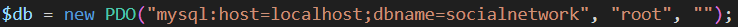
\includegraphics[width=\textwidth]{database1}	
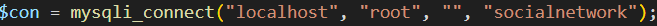
\includegraphics[width=\textwidth]{database2}
\caption{Connexion à la base de données}
\end{figure}\\
Remplacez ”\textbf{socialnetwork}” par le nom que vous avez choisit lors de la création de la base de
données.\\
Bien, maintenant que toutes ces informations sont entre vos mains, le site devrait être prêt pour
quelques tests.\\\\
Dans les prochaines parties, nous vous expliquerons en détails le fonctionnement de toutes les features.
\section{Organisation de notre travail}
Le travail demandé étant conséquent. Nous avons dû nous organiser pour prévenir à d'éventuelles difficultées. Notre projet s'organise autour de 7 dossiers. Nous avons essayé d'être le plus clair possible concernant le nommage des fichiers pour éviter toutes ambiguïtées.
\begin{figure}[h]\centering
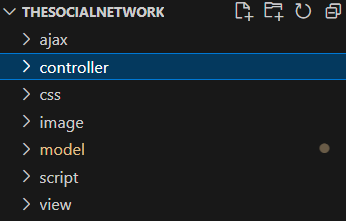
\includegraphics[width=0.5\textwidth]{branche}	
\caption{Arborescence du projet}
\end{figure}\\
Les noms étant assez explicites, nous allons expliquer leur rôle de manière non-exhaustive.\\\\
\textbf{- Dossier View : }\\
Ce dossier regroupe tous les fichiers qui affichent un modules sur le site.\\\\
\textbf{- Dossier script : }\\
Celui-ci regroupe tous les \textbf{scripts} javascript servant à rendre le site plus agréables pour l'utilisateur. On y retrouve par exemple les fichiers servant à envoyer des requêtes AJAX.\\\\
\textbf{- Dossier Model : }\\
Ce dossier regroupe tous les fichiers servant aux traitements des données dans la BDD.\\\\
\textbf{- Dossier Image : }\\
Celui-ci stocke les images des posts, des avatars des utilisateurs et des images des commentaires. Les images ne sont pas stockées dans la BDD mais bien en local.\\\\
\textbf{- Dossier Ajax : }\\
Ce dossier traite toutes les requêtes \textbf{AJAX} côté BDD.\\\\
Concernant le \textbf{versionning} de notre code. Nous avons choisit \href{https://git-scm.com/}{\textbf{Git}}. Vous pouvez trouver le lien de notre répertoire \textbf{Github} sur tous les pieds de pages.
\section{Utilisateurs connectés/déconnectés}
Le but de cette partie est d'expliquer dans les grandes lignes la différence entre les droits accordés aux utilisateurs connectés et ceux non connectés.
\subsection{Utilisateurs déconnectés}
Un utilisateur qui arriverait sur le site pour la première fois pourrait entre autres:
\begin{enumerate}
\item Rechercher dans la barre de recherche un \textbf{utilisateur} ou un \textbf{post} mais sans intéragir avec ceux-ci. Impossibilité de \textbf{liker} et \textbf{commenter} un post et impossibilité de \textbf{suivre} ni même de voir les \textbf{followers} ou les \textbf{following} d'un utilisateur.
\item Les posts marqués comme \textbf{"sensible"} ne peuvent pas être défloutés. Un badge précise qu'il faut avoir un compte et être connecté pour pouvoir faire cette action sur les \textbf{posts concernés}.
\item Les \textbf{commentaires} de chaque post peuvent être \textbf{consultés} mais pas likés.
\end{enumerate}
\subsection{Utilisateurs connectés}
Les utilisateurs connectés ont accès aux fonctionnalités de la liste \textbf{3.1}. En plus de cela, sur sa page, un utilisateur peut changer  ses informations personnelles et consulter les statistiques de son compte.
\subsection{Côté backend}
Côté backend, on le verra plus en détails dans l'explication de chaque feature. Mais le principal pour la connexion  d'un utilisateur est géré via \textbf{des variables de session}.\\\\ 
C'est-à-dire qu'à la connexion ou l'inscription, certaines données sont stockées dans une variable \textbf{SESSION}. Comme par exemple \texttt{\$\_SESSION["id\_user"]}. C'est cette variable qui permet de donner les accès vus en \textbf{3.1} et \textbf{3.2}.\\\\ 
La variable \texttt{\$\_SESSION["admin"]} permet de donner les accès à \textbf{l'administrateur} du réseau social. Il peut flouter et supprimer un post jugé trop violant. Il peut également envoyer un \textbf{avertissement} et \textbf{bannir} un utilisateur. 
\section{S'inscrire / se connecter}
Le centre névralgique de notre site est la \textbf{navbar} située dans le fichier \textbf{./view/navbar.php}. Celle-ci s'affiche sur toutes les pages de notre site sauf pour les pages \textbf{./model/undelete\_page.php} et \textbf{./model/unblur\_page.php} uniquement disponibles pour l'administrateur.
\subsection{Se connecter}
Le backend et le frontend de l'inscription se font dans les fichiers suivant :
\begin{itemize}
\item ./view/popup\_signin.php (définit les "\textbf{divs}" nécessaires au pop-up d'inscription).
\item ./view/form\_signin.html (définit le formulaire pour l'inscription).
\item ./model/signin.php (vérifie les données des "\textbf{input}" rentrées par les utilisateurs: email + mot de passe) 
\item ./css/signin.css (fichier css pour le frontend du signin).
\end{itemize}
\subsubsection{Vérification des données}
Dans cette partie nous allons expliquer en détails le fichier ./model/signin.php.\\\\
L'utilisateur arrive sur le site est clique sur l'icône utilisateur de la navbar. Un popup apparaît (figure 3).
\begin{figure}[h]\centering
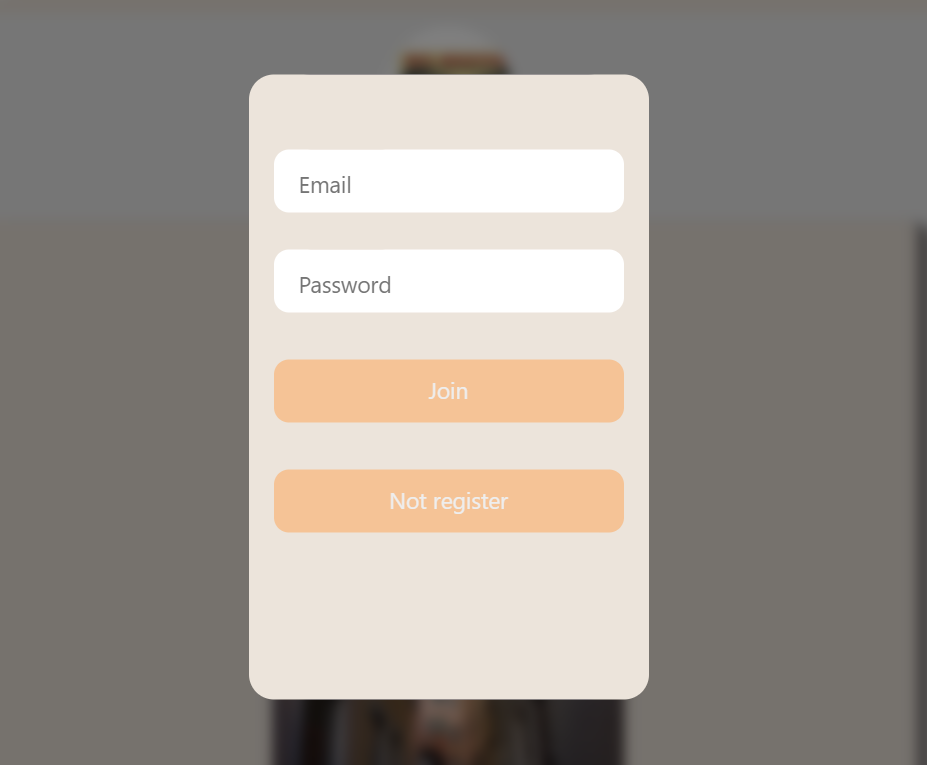
\includegraphics[width=\textwidth]{popup}
\caption{Pop-up de connexion}
\end{figure}\\
Il rentre ses informations et clique sur "join". Les données sont envoyés grâce à la méthode \textbf{POST}. Côté backend, on vérifie si la variable \textbf{\$\_POST} n'est pas vide avec la fonction \textbf{empty()}. Ensuite on \textbf{sécurise} les inputs pour s'abstenir des injections SQL et autres fantaisies.\\\\
On vérifie également que l'email est bien au format attendu même si le "type" de l'input dans le formulaire est "email". Si ce n'est pas le cas on envoie une \textbf{alert} javascript pour prévenir l'utilisateur.\\\\
Une fois que les données sont prêtes à  être exploitées, on effectue une requête à la base de donnée pour voir si l'utilisateur existe. ("SELECT * FROM user WHERE email = \$email"). Si c'est le cas, on vérifie si le "password" est le même. Celui-ci étant "hash" avec la fonction \textbf{password\_hash()}, on utilise une fonction  \textbf{password\_verify()} pour le comparer au "hash" de la BDD.\\\\
Si le mot de passe correspond il ne reste plus qu'à faire une seul vérification.\\\\
Un utilisateur pouvant être \textbf{banni} un nombre de jour choisit entre 0 et 100 par l'administrateur. On se \textbf{doit de vérifier à chaque connexion} la durée restante du "ban" de l'utilisateur. Si celui-ci est concerné, on se doit de le débannir si la durée est arrivée à échéance.\\\\
Une fois toutes ces étapes effectuées. On "set" \textbf{les variables de session} utiles au bon fonctionnement du site. Puis on redirige l'utilisateur vers sa page personnelle. La navbar s'adapte quand l'utilisateur est connecté.
\begin{figure}[!t]\centering
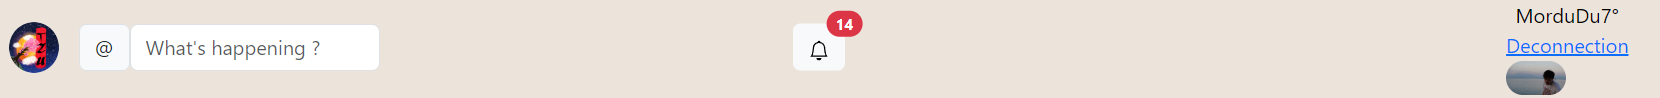
\includegraphics[width=\textwidth]{navbarA}
\caption{Navbar après connexion, les notifications seront alors accessibles sur toutes les pages}
\end{figure}\\
\subsection{S'inscrire}
S'inscrire s'inscrit dans la même dynamique que la connexion. Des informations sont demandées en plus comme une photo de profile qui \textbf{n'est pas obligatoire}, une date d'anniversaire, un nom et un prénom.\\\\
Si aucune photo est choisit une couleur est générée aléatoirement. Un macaron avec la première lettre du prénom sera alors afficher à la place de la photo de profile.\\\\
La gestion du formulaire se situe sur une page à part entière \textbf{./model/signup.php}.
\section{Découvrir des posts/utilisateurs}
La navbar se compose également d'une barre de recherche. Celle-ci permet de rechercher des utilisateurs et des posts en même temps. Deux sections vont alors s'afficher lors de la recherche.
\begin{figure}[h]\centering
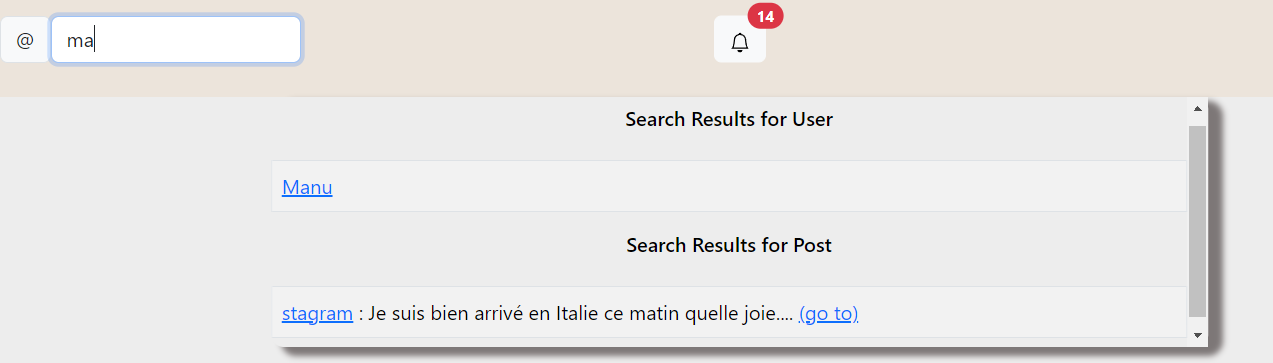
\includegraphics[width=\textwidth]{recherche}
\caption{Recherche}
\end{figure}\\
Cette recherche est complétement gérer via des \textbf{requêtes Ajax}. La requête est créée dans le fichier ./script/ajax\_search.js. Lorsque l'utilisateur \textbf{frappe une touche de son clavier}. Une requête est envoyer au fichier ./ajax/livesearch.php.\\\\
 Ce fichier fait le traitement dans la BDD pour \textbf{rechercher des utilisateurs} dont le pseudo (de manière analogue pour les posts mais cette fois ci sur le "content" du post) est composé des lettres rentrées par l'utilisateur dans la barre de recherche. Si il y a une correspondance, on créé deux tables avec les pseudos et les posts correspondants.\\\\
Lorsque la requête Ajax reçoit le résultat du fichier php. Elle change la \textbf{propriété} de la div "wrap" pour la rendre \textbf{visible} puis elle ajoute à la div "searchresult" contenue dans la div "wrap" les deux tables générées lors du traitement des données de la requête Ajax.\\\\
Dans le cas où il n'y a pas d'utilisateurs ni de posts \textbf{correspondants}. Le résultat de la requête avertira l'utilisateur qu'il n'y a pas d'utilisateurs ou de posts trouvés.
\end{document}	